\documentclass[10pt,x11names,table]{beamer}

\usetheme[progressbar=frametitle]{metropolis}
\usepackage{appendixnumberbeamer}
\usepackage{xcolor}

\usepackage{polyglossia}
\setmainlanguage{spanish}

\usepackage{listings}

\usepackage{booktabs}
\usepackage[scale=2]{ccicons}

\usepackage{pgfplots}
\usepgfplotslibrary{dateplot}

%ANIMACIONES
\usepackage{animate}
\usepackage{graphicx}
\usepackage[caption=false]{subfig}

\usepackage{xspace}

\newcommand*{\eg}{e.g.\@\xspace}
\newcommand*{\ie}{i.e.\@\xspace}

\let\oldquote\quote
\let\endoldquote\endquote
\renewenvironment{quote}[2][]
  {\if\relax\detokenize{#1}\relax
     \def\quoteauthor{#2}%
   \else
     \def\quoteauthor{#2~---~#1}%
   \fi
   \oldquote}
  {\par\nobreak\smallskip\hfill(\quoteauthor)%
   \endoldquote\addvspace{\bigskipamount}}
   
\usepackage{wrapfig}

\usepackage{subfig}
\usepackage{hyperref}
\usepackage{multicol}

\setbeamertemplate{bibliography item}[text]

\usepackage[font=small,skip=0pt, labelformat=empty]{caption}

\usepackage{dirtytalk}
\usepackage[acronym]{glossaries}
\makeglossaries

\newacronym{acgan}{ACGAN}{Auxiliary Classifier GAN}
\newacronym{ae}{AE}{Autoencoder}
\newacronym{ai}{AI}{Artificial Intelligence}
\newacronym{api}{API}{Application Programming Interface}
\newacronym{bert}{BERT}{Bidirectional Encoder Representations from Transformers}
\newacronym{brief}{BRIEF}{Binary Robust Independent Elementary Features}
\newacronym{brnn}{BRNN}{Bidirectional RNN}
\newacronym{bptt}{BPTT}{Backpropagation Through Time}
\newacronym{cbow}{CBOW}{Continous bag-of-words}
\newacronym{cnn}{CNN}{Convolutional Neural Network}
\newacronym{crnn}{CRNN}{Convolutional Recurrent Neural Network}
\newacronym{ddpm}{DDPM}{Denoising Diffusion Probabilistic Model}
\newacronym{ddim}{DDIM}{Denoising Diffusion Implicit Model}
\newacronym{diffit}{DiffiT}{Diffusion Vision Transformer}
\newacronym{dl}{DL}{Deep Learning}
\newacronym{dnn}{DNN}{Deep Neural Network}
\newacronym{dos}{DoS}{Denial of Service}
\newacronym{drnn}{DRNN}{Deep Recurrent Neural Network}
\newacronym{ecg}{ECG}{Electrocardiogram}
\newacronym{elmo}{ELMo}{Embedding from Language Model}
\newacronym{fast}{FAST}{Features from Accelerated Segment Test}
\newacronym{fid}{FID}{Fréchet Inception Distance}
\newacronym{foss}{FOSS}{Free and open-source software}
\newacronym{gan}{GAN}{Generative Adversarial Network}
\newacronym{glove}{GloVe}{Global Vectors for Word Representation}
\newacronym{gpu}{GPU}{Graphics Processing Unit}
\newacronym{gru}{GRU}{Gated Recurrent Unit}
\newacronym{ilsvrc}{ILSVRC}{ImageNet Large Scale Visual Recognition Challenge}
\newacronym{is}{IS}{Inception Score}
\newacronym{kid}{KID}{Kernel Inception Distance}
\newacronym{ldm}{LDM}{Latent Diffusion Model}
\newacronym{lstm}{LSTM}{Long Short-Term Memory}
\newacronym{mape}{MAPE}{Mean Absolute Perentage Error}
\newacronym{ml}{ML}{Machine Learning}
\newacronym{mlp}{MLP}{Multilayer Perceptron}
\newacronym{mmd}{MMD}{Maximum Mean Discrepancy}
\newacronym{mse}{MSE}{Mean Squared Error}
\newacronym{ner}{NER}{Named Entity Recognition}
\newacronym{nlg}{NLG}{Natural Language Generation}
\newacronym{nlp}{NLP}{Natural Language Processing}
\newacronym{nlu}{NLU}{Natural Language Understanding}
\newacronym{nn}{NN}{Neural Network}
\newacronym{ocr}{OCR}{Optical Character Recognition}
\newacronym{onnx}{ONNX}{Open Neural Network Exchange}
\newacronym{pmml}{PMML}{Predictive Model Markup Language}
\newacronym{relu}{ReLU}{Rectified Linear Unit}
\newacronym{rest}{REST}{Representational State Transfer}
\newacronym{rnn}{RNN}{Recurrent Neural Network}
\newacronym{sae}{SAE}{Stacked Autoencoder}
\newacronym{sift}{SIFT}{Scale-Invariant Feature Transform}
\newacronym{slam}{SLAM}{Simultaneous Localization and Mapping}
\newacronym{sru}{SRU}{Single Recurrent Unit}
\newacronym{surf}{SURF}{Speeded-Up Robust Features}
\newacronym{svm}{SVM}{Support Vector Machine}
\newacronym{vae}{VAE}{Variational Autoencoder}
\newacronym{vgg}{VGG}{Visual Geometry Group}
\newacronym{vit}{ViT}{Vision Transformer}
\newacronym{wsgi}{WSGI}{Web Server Gateway Interface}
\newacronym{xai}{XAI}{eXplainable Artificial Intelligence}
\newacronym{yolo}{YOLO}{You Only Look Once}
\newacronym{zsl}{ZSL}{Zero-shot Learning}
\subtitle{Métodos Generativos, curso 2024-2025}

\date{\today}
\author{Guillermo Iglesias, guillermo.iglesias@upm.es \newline
Jorge Dueñas Lerín, jorge.duenas.lerin@upm.es  \newline
Félix Fuentes Hurtado, felix.fuentes@upm.es}

\institute{Escuela Técnica Superior de Ingeniería de Sistemas Informáticos | UPM \newline
\hbox{} \newline \ccbysa \hspace{0.1pt} \ccNonCommercial}

%%%%%%%%%%%%%%%%%%%%%%%%%%%%%%%%%%%%%       
\title{Redes convolucionales II}

\begin{document}
\maketitle

\begin{frame}{Construcción de una \gls{cnn}}
La estructura de \alert{embudo} típica de las redes neuronales \alert{clasificadoras} también se aplica a \gls{cnn}. Para ello el objetivo es \alert{reducir} la dimensión de la imagen hasta generar una salida.

\begin{figure}
    \centering
    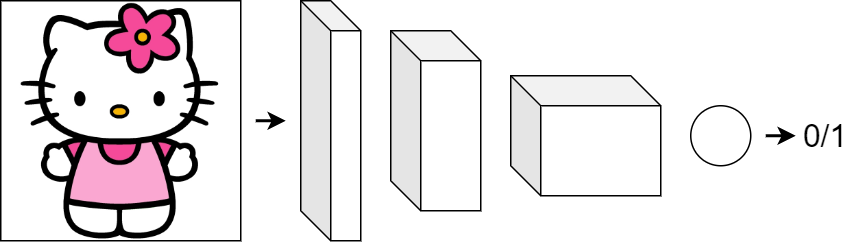
\includegraphics[width=\textwidth]{Slides/figures/Tema 3/CNNEmbudo.png}
\end{figure}
\end{frame}

\begin{frame}{Construcción de una \gls{cnn}}
Las primeras capas \alert{convolucionales} de la red se encargan de la \alert{extracción de características} de la imagen. Posteriormente un \alert{perceptrón} se encarga de \alert{clasificar} las características extraídas para generar la \alert{salida deseada}.

\begin{figure}
    \centering
    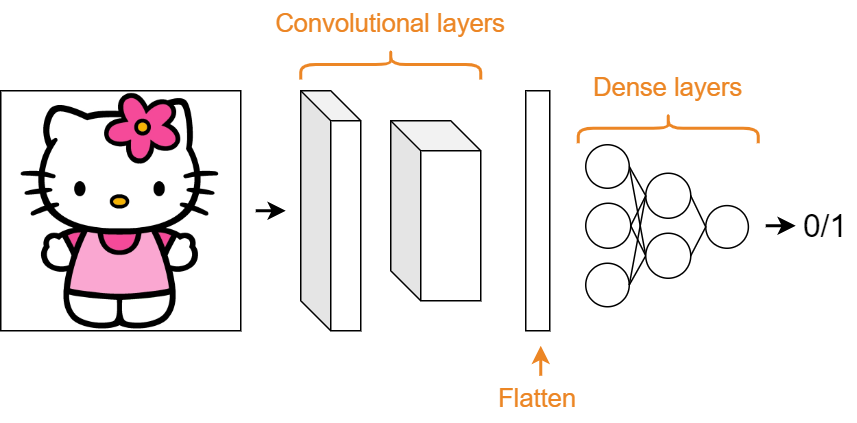
\includegraphics[width=\textwidth]{Slides/figures/Tema 3/CNNPerceptron.png}
\end{figure}
\end{frame}

\begin{frame}{Construcción de una \gls{cnn}}
Es importante recordar que la \alert{jerarquía} de capas de una red convolucional detecta características a \alert{alto nivel} en las capas \alert{más profundas}.

\begin{figure}
    \centering
    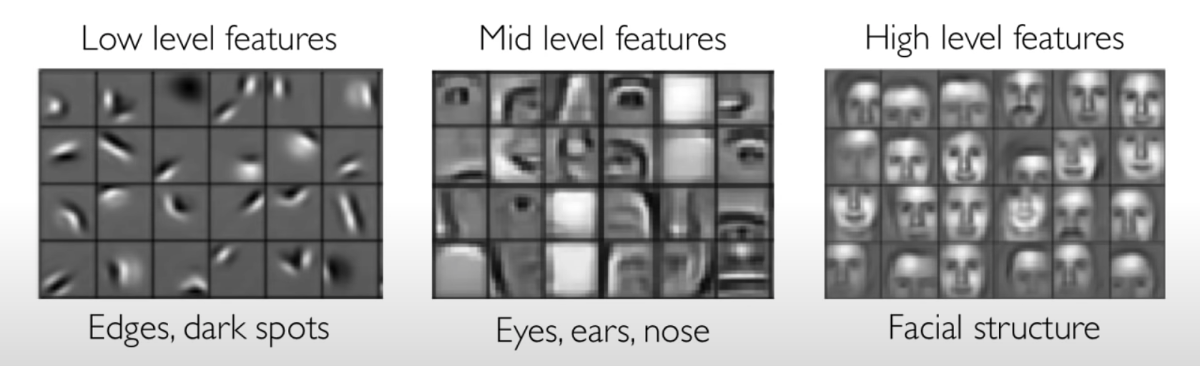
\includegraphics[width=\textwidth]{Slides/figures/Tema 3/ConvHierarchy_1.png}
    \caption{\cite{ConvHierarchy}}
\end{figure}
\end{frame}

\begin{frame}{Reducción dimensional en redes convolucionales}
Para formar el \say{\alert{embudo}} de la red se utilizan distintos mecanismos para \alert{reducir las dimensiones} de la información de la red. En concreto los dos mecanismos predominantes son:
\begin{itemize}
    \item \alert{Capas de pooling}
    \begin{itemize}
        \item MaxPooling
        \item AveragePooling
    \end{itemize}
    \item \alert{Convoluciones de strides=(2,2)}
\end{itemize}
\end{frame}

\begin{frame}{Reducción dimensional con Pooling}
\alert{\Large MaxPooling 2D}
La capa de MaxPooling2D reduce la dimensión de un vector cogiendo el \alert{máximo} de la ventana definida.

\begin{figure}
    \centering
    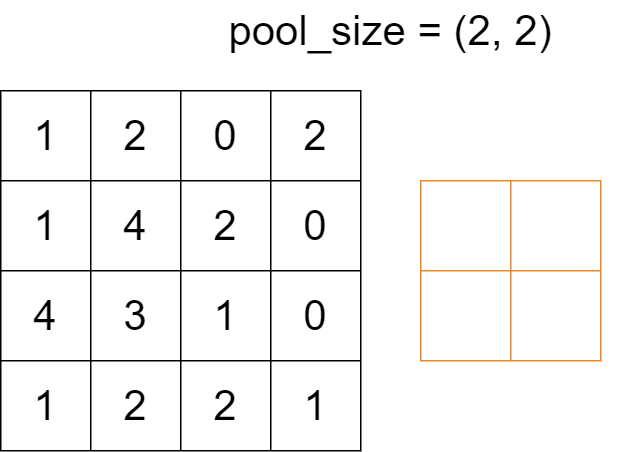
\includegraphics[width=0.7\textwidth]{Slides/figures/Tema 3/MaxPooling_1.png}
\end{figure}
\end{frame}

\begin{frame}{Reducción dimensional con Pooling}
\alert{\Large MaxPooling 2D}
La capa de MaxPooling2D reduce la dimensión de un vector cogiendo el \alert{máximo} de la ventana definida.

\begin{figure}
    \centering
    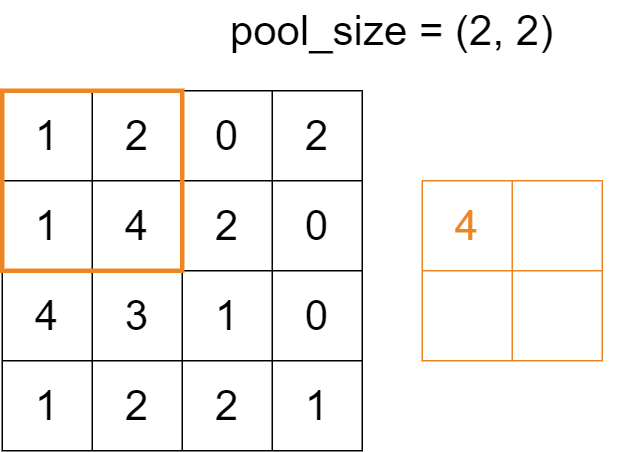
\includegraphics[width=0.7\textwidth]{Slides/figures/Tema 3/MaxPooling_2.png}
\end{figure}
\end{frame}

\begin{frame}{Reducción dimensional con Pooling}
\alert{\Large MaxPooling 2D}
La capa de MaxPooling2D reduce la dimensión de un vector cogiendo el \alert{máximo} de la ventana definida.

\begin{figure}
    \centering
    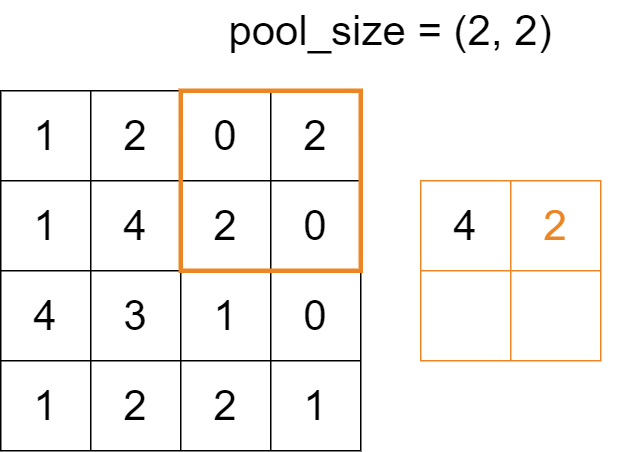
\includegraphics[width=0.7\textwidth]{Slides/figures/Tema 3/MaxPooling_3.png}
\end{figure}
\end{frame}

\begin{frame}{Reducción dimensional con Pooling}
\alert{\Large MaxPooling 2D}
La capa de MaxPooling2D reduce la dimensión de un vector cogiendo el \alert{máximo} de la ventana definida.

\begin{figure}
    \centering
    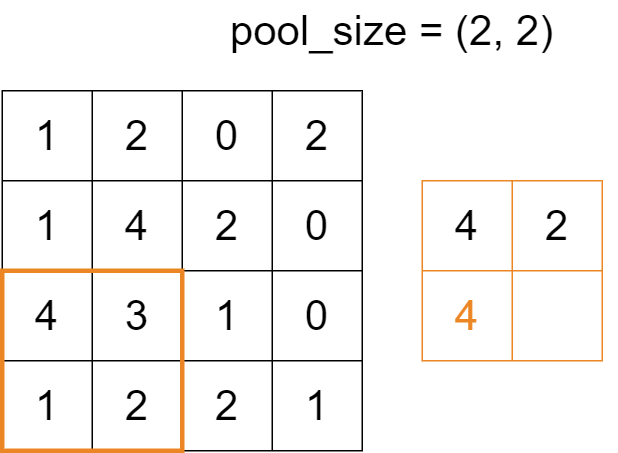
\includegraphics[width=0.7\textwidth]{Slides/figures/Tema 3/MaxPooling_4.png}
\end{figure}
\end{frame}

\begin{frame}{Reducción dimensional con Pooling}
\alert{\Large MaxPooling 2D}
La capa de MaxPooling2D reduce la dimensión de un vector cogiendo el \alert{máximo} de la ventana definida.

\begin{figure}
    \centering
    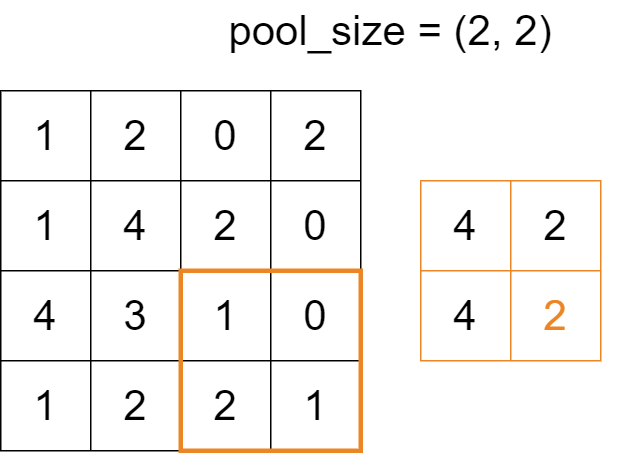
\includegraphics[width=0.7\textwidth]{Slides/figures/Tema 3/MaxPooling_5.png}
\end{figure}
\end{frame}

\begin{frame}{Reducción dimensional con Pooling}
\alert{\Large MaxPooling 2D}
La capa de MaxPooling2D reduce la dimensión de un vector cogiendo el \alert{máximo} de la ventana definida.

\begin{figure}
    \centering
    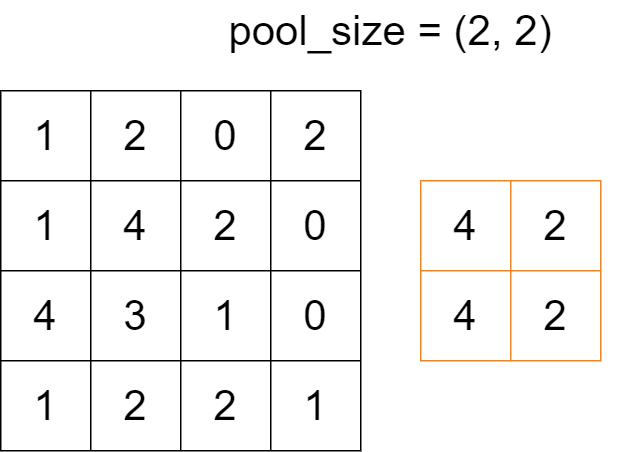
\includegraphics[width=0.7\textwidth]{Slides/figures/Tema 3/MaxPooling_res.png}
\end{figure}
\textit{*cabe destacar que el máximo se encarga de preservar la característica más importante}
\end{frame}

\begin{frame}{Reducción dimensional con Pooling}
\alert{\Large AveragePooling 2D}
La capa de AveragePooling2D reduce la dimensión de un vector cogiendo el \alert{promedio} de la ventana definida.

\begin{figure}
    \centering
    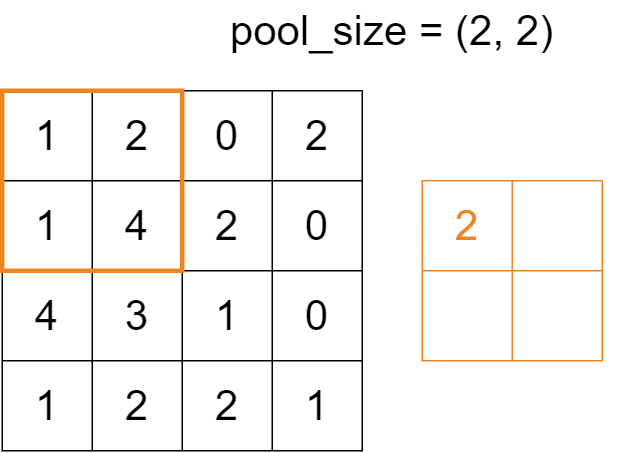
\includegraphics[width=0.7\textwidth]{Slides/figures/Tema 3/AvgPooling_1.png}
\end{figure}
\end{frame}

\begin{frame}{Reducción dimensional con Pooling}
\alert{\Large AveragePooling 2D}
La capa de AveragePooling2D reduce la dimensión de un vector cogiendo el \alert{promedio} de la ventana definida.

\begin{figure}
    \centering
    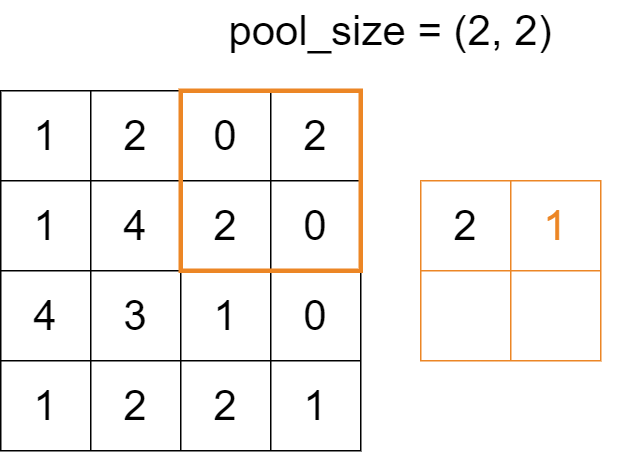
\includegraphics[width=0.7\textwidth]{Slides/figures/Tema 3/AvgPooling_2.png}
\end{figure}
\end{frame}

\begin{frame}{Reducción dimensional con Pooling}
\alert{\Large AveragePooling 2D}
La capa de AveragePooling2D reduce la dimensión de un vector cogiendo el \alert{promedio} de la ventana definida\footnote{Pese a su similitar rendimiento, el MaxPooling suele generar mejores resultados que el AveragePooling \cite{bieder2021comparison}}.

\begin{figure}
    \centering
    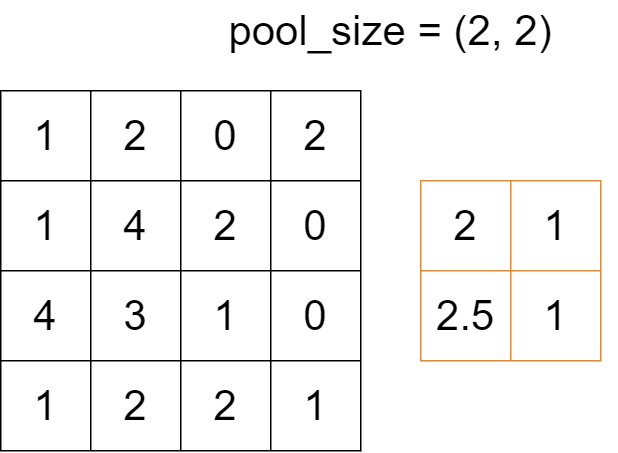
\includegraphics[width=0.7\textwidth]{Slides/figures/Tema 3/AvgPooling_res.png}
\end{figure}
\end{frame}

\begin{frame}{Reducción dimensional con strides}
Otra \alert{alternativa} para la reducción dimensional es el uso de convoluciones con \alert{strides} que no sean (1, 1). Cierta literatura apunta a esta aproximación como \say{\alert{más inteligente}} ya que se le permite a la \alert{red} que sea ella la que escoja \alert{cómo hacer} la reducción.

El principal \alert{inconveniente} es que usando este método se aumenta el número de parámetros de la red.

Existe cierto debate si es conveniente que la red \alert{aprenda} ha hacer el downsampling \cite{MaxPoolingvsStrides} o usar MaxPooling \cite{sun2018fishnet}.

\textit{*Normalmente el stride elegido es de (2, 2) pero hay libertad para adaptarlo a distintos casos.}
\end{frame}

\begin{frame}{Capa de dropout}
La capa de \alert{dropout} es una capa de \alert{regularización} que \alert{desactiva aleatoriamente} la activación de ciertas \alert{neuronas} durante el entreno.

Al regularizar la red previene de problemas como el \alert{overfitting}.

\begin{figure}
    \centering
    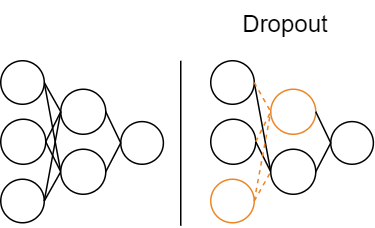
\includegraphics[width=0.7\textwidth]{Slides/figures/Tema 3/Dropout.png}
\end{figure}
\end{frame}

\section{Tuneo de \glspl{cnn}}

\begin{frame}{Los hiperparámetros en una red}
Uno de los mayores \alert{inconvenientes} a la hora de realizar entrenamientos con redes neuronales artificiales es su \alert{difícil configuración}. Debido a la cantidad inmensa de \alert{hiperparámetros} a escoger.

Sin embargo, existen una serie de \alert{prácticas comunes} a la hora de tratar con \glspl{cnn}.
\end{frame}

\begin{frame}{Tamaño de imagen y filtros}
A la hora de escoger el \alert{número de filtros} de cada capa convolucional este va \alert{ligado} al tamaño de la \alert{matriz de datos}.

A medida que la imagen de entrada va \alert{reduciendo} su tamaño, el número de filtros \alert{aumenta}. Con esto se pretende extraer más \alert{características de alto nivel} cada vez cubriendo zonas más amplias de la imagen original.

\begin{figure}
    \centering
    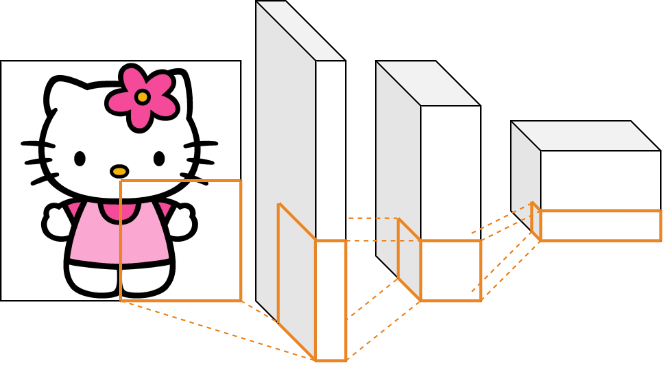
\includegraphics[width=0.7\textwidth]{Slides/figures/Tema 3/DimensionFilters.png}
\end{figure}
\end{frame}

\begin{frame}{Tamaño de imagen y filtros}
Al mismo tiempo, a medida que el \alert{número} de filtros de \alert{multiplica por 2} las \alert{dimensiones} de la matriz de datos se \alert{reducen a la mitad}.

El objetivo de este \alert{intercambio} es mantener la \alert{misma cantidad} de información, pero tratada por la red.

\begin{figure}
    \centering
    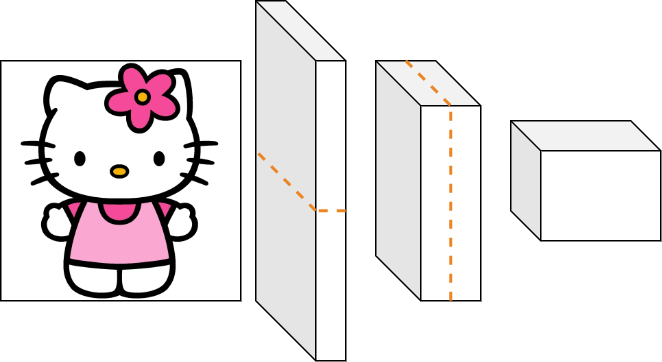
\includegraphics[width=0.7\textwidth]{Slides/figures/Tema 3/ResolutionFilter_1.png}
\end{figure}
\end{frame}

\begin{frame}{Otros hiperparámetros}
\alert{\Large kernel\_size}

El tamaño del kernel \alert{habitualmente} es de \alert{(3, 3)} o \alert{(5, 5)}, en caso de imágenes muy grandes puede llegar a \alert{(7, 7)}.

Para matrices de datos \alert{más grandes} se utilizan \alert{kernels más grandes}, en casos combinando kernels de \alert{(5, 5)} para las \alert{primeras capas} y posteriormente \alert{(3, 3)} para capas más \alert{profundas}\footnote{Investigaciones posteriores \cite{simonyan2014very} han demostrado que es más eficiente apilar dos capas convoluciones de (3, 3) que una única capa de (5, 5).}.

\vfill
\alert{\Large strides}

El paso de la convolución se mantiene a \alert{(1, 1)} a no ser que se desee una \alert{reducción dimensional}.
\end{frame}

\begin{frame}{Otros hiperparámetros}
\alert{\Large padding}

El padding de una convolución suele ser \alert{same} para controlar las dimensiones de la matriz de datos, pero no es extraño encontrar casos con padding \alert{valid}.

\vfill
\alert{\Large activation}

Para las \alert{capas ocultas} se suele utilizar la función \alert{ReLU} o \alert{LeakyReLU}, para la capa de \alert{salida} la activación depende del \alert{problema concreto}.
\end{frame}

\begin{frame}{Ejemplo}
    \centering
    
\includegraphics[width=0.4\textwidth]{Slides/figures/GoogleColab.png}
\begin{itemize}
    \centering
    \item {\Large \href{https://colab.research.google.com/drive/17QwnRs7P0bv6kYsbQPYIrIDjk-uL_9rd?usp=sharing}{1.2\_2-CNNEmbudo.ipynb}}
\end{itemize}
\end{frame}

\addcontentsline{toc}{section}{Referencias}

\begin{frame}[allowframebreaks]{Referencias}
    \bibliographystyle{unsrt}
    \bibliography{Slides/references.bib}
\end{frame}

\begin{frame}{Contribuciones de las diapositivas}
\begin{itemize}
    \item \textbf{Autor original de las diapositivas:} Guillermo Iglesias Hernández
\end{itemize}
\end{frame}

\end{document}